\documentclass[twoside]{book}

% Packages required by doxygen
\usepackage{fixltx2e}
\usepackage{calc}
\usepackage{doxygen}
\usepackage[export]{adjustbox} % also loads graphicx
\usepackage{graphicx}
\usepackage[utf8]{inputenc}
\usepackage{makeidx}
\usepackage{multicol}
\usepackage{multirow}
\PassOptionsToPackage{warn}{textcomp}
\usepackage{textcomp}
\usepackage[nointegrals]{wasysym}
\usepackage[table]{xcolor}

% Font selection
\usepackage[T1]{fontenc}
\usepackage[scaled=.90]{helvet}
\usepackage{courier}
\usepackage{amssymb}
\usepackage{sectsty}
\renewcommand{\familydefault}{\sfdefault}
\allsectionsfont{%
  \fontseries{bc}\selectfont%
  \color{darkgray}%
}
\renewcommand{\DoxyLabelFont}{%
  \fontseries{bc}\selectfont%
  \color{darkgray}%
}
\newcommand{\+}{\discretionary{\mbox{\scriptsize$\hookleftarrow$}}{}{}}

% Page & text layout
\usepackage{geometry}
\geometry{%
  a4paper,%
  top=2.5cm,%
  bottom=2.5cm,%
  left=2.5cm,%
  right=2.5cm%
}
\tolerance=750
\hfuzz=15pt
\hbadness=750
\setlength{\emergencystretch}{15pt}
\setlength{\parindent}{0cm}
\setlength{\parskip}{3ex plus 2ex minus 2ex}
\makeatletter
\renewcommand{\paragraph}{%
  \@startsection{paragraph}{4}{0ex}{-1.0ex}{1.0ex}{%
    \normalfont\normalsize\bfseries\SS@parafont%
  }%
}
\renewcommand{\subparagraph}{%
  \@startsection{subparagraph}{5}{0ex}{-1.0ex}{1.0ex}{%
    \normalfont\normalsize\bfseries\SS@subparafont%
  }%
}
\makeatother

% Headers & footers
\usepackage{fancyhdr}
\pagestyle{fancyplain}
\fancyhead[LE]{\fancyplain{}{\bfseries\thepage}}
\fancyhead[CE]{\fancyplain{}{}}
\fancyhead[RE]{\fancyplain{}{\bfseries\leftmark}}
\fancyhead[LO]{\fancyplain{}{\bfseries\rightmark}}
\fancyhead[CO]{\fancyplain{}{}}
\fancyhead[RO]{\fancyplain{}{\bfseries\thepage}}
\fancyfoot[LE]{\fancyplain{}{}}
\fancyfoot[CE]{\fancyplain{}{}}
\fancyfoot[RE]{\fancyplain{}{\bfseries\scriptsize Generated by Doxygen }}
\fancyfoot[LO]{\fancyplain{}{\bfseries\scriptsize Generated by Doxygen }}
\fancyfoot[CO]{\fancyplain{}{}}
\fancyfoot[RO]{\fancyplain{}{}}
\renewcommand{\footrulewidth}{0.4pt}
\renewcommand{\chaptermark}[1]{%
  \markboth{#1}{}%
}
\renewcommand{\sectionmark}[1]{%
  \markright{\thesection\ #1}%
}

% Indices & bibliography
\usepackage{natbib}
\usepackage[titles]{tocloft}
\setcounter{tocdepth}{3}
\setcounter{secnumdepth}{5}
\makeindex

% Hyperlinks (required, but should be loaded last)
\usepackage{ifpdf}
\ifpdf
  \usepackage[pdftex,pagebackref=true]{hyperref}
\else
  \usepackage[ps2pdf,pagebackref=true]{hyperref}
\fi
\hypersetup{%
  colorlinks=true,%
  linkcolor=blue,%
  citecolor=blue,%
  unicode%
}

% Custom commands
\newcommand{\clearemptydoublepage}{%
  \newpage{\pagestyle{empty}\cleardoublepage}%
}

\usepackage{caption}
\captionsetup{labelsep=space,justification=centering,font={bf},singlelinecheck=off,skip=4pt,position=top}

%===== C O N T E N T S =====

\begin{document}

% Titlepage & ToC
\hypersetup{pageanchor=false,
             bookmarksnumbered=true,
             pdfencoding=unicode
            }
\pagenumbering{roman}
\begin{titlepage}
\vspace*{7cm}
\begin{center}%
{\Large x\+P\+L\+O\+R\+ER }\\
\vspace*{1cm}
{\large Generated by Doxygen 1.8.11}\\
\end{center}
\end{titlepage}
\clearemptydoublepage
\tableofcontents
\clearemptydoublepage
\pagenumbering{arabic}
\hypersetup{pageanchor=true}

%--- Begin generated contents ---
\chapter{Class Index}
\section{Class List}
Here are the classes, structs, unions and interfaces with brief descriptions\+:\begin{DoxyCompactList}
\item\contentsline{section}{\hyperlink{classnavigator}{navigator} \\*Class for navigation part of the robot }{\pageref{classnavigator}}{}
\item\contentsline{section}{\hyperlink{classobstacleDetector}{obstacle\+Detector} \\*Class for obstacle\+Detection part of the robot }{\pageref{classobstacleDetector}}{}
\item\contentsline{section}{\hyperlink{classTestClass}{Test\+Class} \\*Class for testing }{\pageref{classTestClass}}{}
\end{DoxyCompactList}

\chapter{File Index}
\section{File List}
Here is a list of all documented files with brief descriptions\+:\begin{DoxyCompactList}
\item\contentsline{section}{/home/akash/catkin\+\_\+ws/src/x\+P\+L\+O\+R\+E\+R/include/xplorer/\hyperlink{navigator_8hpp}{navigator.\+hpp} \\*\subsection*{\+: Class implementation for Robot Navigation functionality }}{\pageref{navigator_8hpp}}{}
\item\contentsline{section}{/home/akash/catkin\+\_\+ws/src/x\+P\+L\+O\+R\+E\+R/include/xplorer/\hyperlink{obstacleDetector_8hpp}{obstacle\+Detector.\+hpp} \\*\subsection*{\+: Class implementation for obstacle detection functionality }}{\pageref{obstacleDetector_8hpp}}{}
\item\contentsline{section}{/home/akash/catkin\+\_\+ws/src/x\+P\+L\+O\+R\+E\+R/src/\hyperlink{navigator_8cpp}{navigator.\+cpp} \\*\subsection*{\+: Functional implementation for Robot Navigation functionality }}{\pageref{navigator_8cpp}}{}
\item\contentsline{section}{/home/akash/catkin\+\_\+ws/src/x\+P\+L\+O\+R\+E\+R/src/\hyperlink{obstacleDetector_8cpp}{obstacle\+Detector.\+cpp} \\*\subsection*{\+: Functional implementation for obstacle detection functionality }}{\pageref{obstacleDetector_8cpp}}{}
\item\contentsline{section}{/home/akash/catkin\+\_\+ws/src/x\+P\+L\+O\+R\+E\+R/test/\hyperlink{testNavigator_8cpp}{test\+Navigator.\+cpp} \\*\subsection*{\+: Test file for testing class Navigator }}{\pageref{testNavigator_8cpp}}{}
\item\contentsline{section}{/home/akash/catkin\+\_\+ws/src/x\+P\+L\+O\+R\+E\+R/test/\hyperlink{testObstacleDetector_8cpp}{test\+Obstacle\+Detector.\+cpp} \\*\subsection*{\+: Test file for testing class \hyperlink{classobstacleDetector}{obstacle\+Detector} }}{\pageref{testObstacleDetector_8cpp}}{}
\end{DoxyCompactList}

\chapter{Class Documentation}
\hypertarget{classnavigator}{}\section{navigator Class Reference}
\label{classnavigator}\index{navigator@{navigator}}


Class for navigation part of the robot.  




{\ttfamily \#include $<$navigator.\+hpp$>$}



Collaboration diagram for navigator\+:
\nopagebreak
\begin{figure}[H]
\begin{center}
\leavevmode
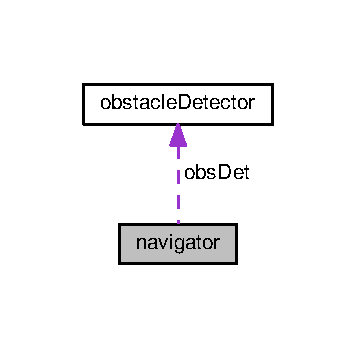
\includegraphics[width=171pt]{classnavigator__coll__graph}
\end{center}
\end{figure}
\subsection*{Public Member Functions}
\begin{DoxyCompactItemize}
\item 
\hyperlink{classnavigator_a56f8f7c47b89e2496a6c95155f163f4a}{navigator} ()\hypertarget{classnavigator_a56f8f7c47b89e2496a6c95155f163f4a}{}\label{classnavigator_a56f8f7c47b89e2496a6c95155f163f4a}

\begin{DoxyCompactList}\small\item\em Constructor. \end{DoxyCompactList}\item 
\hyperlink{classnavigator_a3f3e027d3b440b100426abb9aba16b5e}{$\sim$navigator} ()\hypertarget{classnavigator_a3f3e027d3b440b100426abb9aba16b5e}{}\label{classnavigator_a3f3e027d3b440b100426abb9aba16b5e}

\begin{DoxyCompactList}\small\item\em Destructor. \end{DoxyCompactList}\item 
void \hyperlink{classnavigator_abe0798d499bb9cbd606fa5a398c863cb}{explore} (int flag)
\begin{DoxyCompactList}\small\item\em Function to move the robot. \end{DoxyCompactList}\end{DoxyCompactItemize}
\subsection*{Public Attributes}
\begin{DoxyCompactItemize}
\item 
\hyperlink{classobstacleDetector}{obstacle\+Detector} {\bfseries obs\+Det}\hypertarget{classnavigator_adf30c28ffd5b02114e7ff429afed9892}{}\label{classnavigator_adf30c28ffd5b02114e7ff429afed9892}

\end{DoxyCompactItemize}


\subsection{Detailed Description}
Class for navigation part of the robot. 

\subsection{Member Function Documentation}
\index{navigator@{navigator}!explore@{explore}}
\index{explore@{explore}!navigator@{navigator}}
\subsubsection[{\texorpdfstring{explore(int flag)}{explore(int flag)}}]{\setlength{\rightskip}{0pt plus 5cm}void navigator\+::explore (
\begin{DoxyParamCaption}
\item[{int}]{flag}
\end{DoxyParamCaption}
)}\hypertarget{classnavigator_abe0798d499bb9cbd606fa5a398c863cb}{}\label{classnavigator_abe0798d499bb9cbd606fa5a398c863cb}


Function to move the robot. 


\begin{DoxyParams}{Parameters}
{\em flag} & for operation \\
\hline
\end{DoxyParams}
\begin{DoxyReturn}{Returns}
void 
\end{DoxyReturn}


The documentation for this class was generated from the following files\+:\begin{DoxyCompactItemize}
\item 
/home/akash/catkin\+\_\+ws/src/x\+P\+L\+O\+R\+E\+R/include/xplorer/\hyperlink{navigator_8hpp}{navigator.\+hpp}\item 
/home/akash/catkin\+\_\+ws/src/x\+P\+L\+O\+R\+E\+R/src/\hyperlink{navigator_8cpp}{navigator.\+cpp}\end{DoxyCompactItemize}

\hypertarget{classobstacleDetector}{}\section{obstacle\+Detector Class Reference}
\label{classobstacleDetector}\index{obstacle\+Detector@{obstacle\+Detector}}


Class for obstacle\+Detection part of the robot.  




{\ttfamily \#include $<$obstacle\+Detector.\+hpp$>$}

\subsection*{Public Member Functions}
\begin{DoxyCompactItemize}
\item 
\hyperlink{classobstacleDetector_a097bd0bdd72d1bc17d167a902f0e85c7}{obstacle\+Detector} ()\hypertarget{classobstacleDetector_a097bd0bdd72d1bc17d167a902f0e85c7}{}\label{classobstacleDetector_a097bd0bdd72d1bc17d167a902f0e85c7}

\begin{DoxyCompactList}\small\item\em Constructor of the class. \end{DoxyCompactList}\item 
\hyperlink{classobstacleDetector_af3e934355f1046a3f235cf680817a590}{$\sim$obstacle\+Detector} ()\hypertarget{classobstacleDetector_af3e934355f1046a3f235cf680817a590}{}\label{classobstacleDetector_af3e934355f1046a3f235cf680817a590}

\begin{DoxyCompactList}\small\item\em Destructor of the class. \end{DoxyCompactList}\item 
void \hyperlink{classobstacleDetector_ae12f2ef16507c879349cbaafbe4254e1}{sensor\+Callback} (const sensor\+\_\+msgs\+::\+Laser\+Scan\+::\+Const\+Ptr \&msg)
\begin{DoxyCompactList}\small\item\em Callback function for subscriber to laser\+Scan messages. \end{DoxyCompactList}\item 
void \hyperlink{classobstacleDetector_a3adcedcf00c41fc0ba6e8d97e322f0ee}{sensor\+Callback\+Dist} (const std\+\_\+msgs\+::\+Float64\+::\+Const\+Ptr \&msg)
\begin{DoxyCompactList}\small\item\em Callback function for subscriber to /dist topic. \end{DoxyCompactList}\item 
bool \hyperlink{classobstacleDetector_a90c1101b6e3b4f26251d67793d41bd9c}{collision\+Detect} ()
\begin{DoxyCompactList}\small\item\em Function for returning value of collision flag. \end{DoxyCompactList}\end{DoxyCompactItemize}


\subsection{Detailed Description}
Class for obstacle\+Detection part of the robot. 

\subsection{Member Function Documentation}
\index{obstacle\+Detector@{obstacle\+Detector}!collision\+Detect@{collision\+Detect}}
\index{collision\+Detect@{collision\+Detect}!obstacle\+Detector@{obstacle\+Detector}}
\subsubsection[{\texorpdfstring{collision\+Detect()}{collisionDetect()}}]{\setlength{\rightskip}{0pt plus 5cm}bool obstacle\+Detector\+::collision\+Detect (
\begin{DoxyParamCaption}
{}
\end{DoxyParamCaption}
)}\hypertarget{classobstacleDetector_a90c1101b6e3b4f26251d67793d41bd9c}{}\label{classobstacleDetector_a90c1101b6e3b4f26251d67793d41bd9c}


Function for returning value of collision flag. 


\begin{DoxyParams}{Parameters}
{\em none} & \\
\hline
\end{DoxyParams}
\begin{DoxyReturn}{Returns}
bool collision flag value 
\end{DoxyReturn}
\index{obstacle\+Detector@{obstacle\+Detector}!sensor\+Callback@{sensor\+Callback}}
\index{sensor\+Callback@{sensor\+Callback}!obstacle\+Detector@{obstacle\+Detector}}
\subsubsection[{\texorpdfstring{sensor\+Callback(const sensor\+\_\+msgs\+::\+Laser\+Scan\+::\+Const\+Ptr \&msg)}{sensorCallback(const sensor_msgs::LaserScan::ConstPtr &msg)}}]{\setlength{\rightskip}{0pt plus 5cm}void obstacle\+Detector\+::sensor\+Callback (
\begin{DoxyParamCaption}
\item[{const sensor\+\_\+msgs\+::\+Laser\+Scan\+::\+Const\+Ptr \&}]{msg}
\end{DoxyParamCaption}
)}\hypertarget{classobstacleDetector_ae12f2ef16507c879349cbaafbe4254e1}{}\label{classobstacleDetector_ae12f2ef16507c879349cbaafbe4254e1}


Callback function for subscriber to laser\+Scan messages. 

Callback function for /scan topic.


\begin{DoxyParams}{Parameters}
{\em msg} & Message over the topic /scan \\
\hline
\end{DoxyParams}
\begin{DoxyReturn}{Returns}
void 
\end{DoxyReturn}
\index{obstacle\+Detector@{obstacle\+Detector}!sensor\+Callback\+Dist@{sensor\+Callback\+Dist}}
\index{sensor\+Callback\+Dist@{sensor\+Callback\+Dist}!obstacle\+Detector@{obstacle\+Detector}}
\subsubsection[{\texorpdfstring{sensor\+Callback\+Dist(const std\+\_\+msgs\+::\+Float64\+::\+Const\+Ptr \&msg)}{sensorCallbackDist(const std_msgs::Float64::ConstPtr &msg)}}]{\setlength{\rightskip}{0pt plus 5cm}void obstacle\+Detector\+::sensor\+Callback\+Dist (
\begin{DoxyParamCaption}
\item[{const std\+\_\+msgs\+::\+Float64\+::\+Const\+Ptr \&}]{msg}
\end{DoxyParamCaption}
)}\hypertarget{classobstacleDetector_a3adcedcf00c41fc0ba6e8d97e322f0ee}{}\label{classobstacleDetector_a3adcedcf00c41fc0ba6e8d97e322f0ee}


Callback function for subscriber to /dist topic. 

Callback function for /dist topic.


\begin{DoxyParams}{Parameters}
{\em msg} & Message over the topic /dist \\
\hline
\end{DoxyParams}
\begin{DoxyReturn}{Returns}
void 
\end{DoxyReturn}


The documentation for this class was generated from the following files\+:\begin{DoxyCompactItemize}
\item 
/home/rishchou/catkin\+\_\+ws/src/x\+P\+L\+O\+R\+E\+R/include/xplorer/\hyperlink{obstacleDetector_8hpp}{obstacle\+Detector.\+hpp}\item 
/home/rishchou/catkin\+\_\+ws/src/x\+P\+L\+O\+R\+E\+R/src/\hyperlink{obstacleDetector_8cpp}{obstacle\+Detector.\+cpp}\end{DoxyCompactItemize}

\hypertarget{classTestClass}{}\section{Test\+Class Class Reference}
\label{classTestClass}\index{Test\+Class@{Test\+Class}}


Class for testing.  


\subsection*{Public Member Functions}
\begin{DoxyCompactItemize}
\item 
void \hyperlink{classTestClass_a32e3eabd238e69e5d6b9f5e820fcfb7b}{publish} (const geometry\+\_\+msgs\+::\+Twist\+::\+Const\+Ptr \&msg)
\begin{DoxyCompactList}\small\item\em Temporary callback function. \end{DoxyCompactList}\end{DoxyCompactItemize}


\subsection{Detailed Description}
Class for testing. 

\subsection{Member Function Documentation}
\index{Test\+Class@{Test\+Class}!publish@{publish}}
\index{publish@{publish}!Test\+Class@{Test\+Class}}
\subsubsection[{\texorpdfstring{publish(const geometry\+\_\+msgs\+::\+Twist\+::\+Const\+Ptr \&msg)}{publish(const geometry_msgs::Twist::ConstPtr &msg)}}]{\setlength{\rightskip}{0pt plus 5cm}void Test\+Class\+::publish (
\begin{DoxyParamCaption}
\item[{const geometry\+\_\+msgs\+::\+Twist\+::\+Const\+Ptr \&}]{msg}
\end{DoxyParamCaption}
)\hspace{0.3cm}{\ttfamily [inline]}}\hypertarget{classTestClass_a32e3eabd238e69e5d6b9f5e820fcfb7b}{}\label{classTestClass_a32e3eabd238e69e5d6b9f5e820fcfb7b}


Temporary callback function. 


\begin{DoxyParams}{Parameters}
{\em msg} & Temporary message \\
\hline
\end{DoxyParams}
\begin{DoxyReturn}{Returns}
void 
\end{DoxyReturn}


The documentation for this class was generated from the following file\+:\begin{DoxyCompactItemize}
\item 
/home/akash/catkin\+\_\+ws/src/x\+P\+L\+O\+R\+E\+R/test/\hyperlink{testNavigator_8cpp}{test\+Navigator.\+cpp}\end{DoxyCompactItemize}

\chapter{File Documentation}
\hypertarget{navigator_8hpp}{}\section{/home/rishchou/catkin\+\_\+ws/src/x\+P\+L\+O\+R\+E\+R/include/xplorer/navigator.hpp File Reference}
\label{navigator_8hpp}\index{/home/rishchou/catkin\+\_\+ws/src/x\+P\+L\+O\+R\+E\+R/include/xplorer/navigator.\+hpp@{/home/rishchou/catkin\+\_\+ws/src/x\+P\+L\+O\+R\+E\+R/include/xplorer/navigator.\+hpp}}


\subsection*{\+: Class implementation for Robot Navigation functionality } 


{\ttfamily \#include \char`\"{}geometry\+\_\+msgs/\+Twist.\+h\char`\"{}}\\*
{\ttfamily \#include \char`\"{}obstacle\+Detector.\+hpp\char`\"{}}\\*
Include dependency graph for navigator.\+hpp\+:
\nopagebreak
\begin{figure}[H]
\begin{center}
\leavevmode
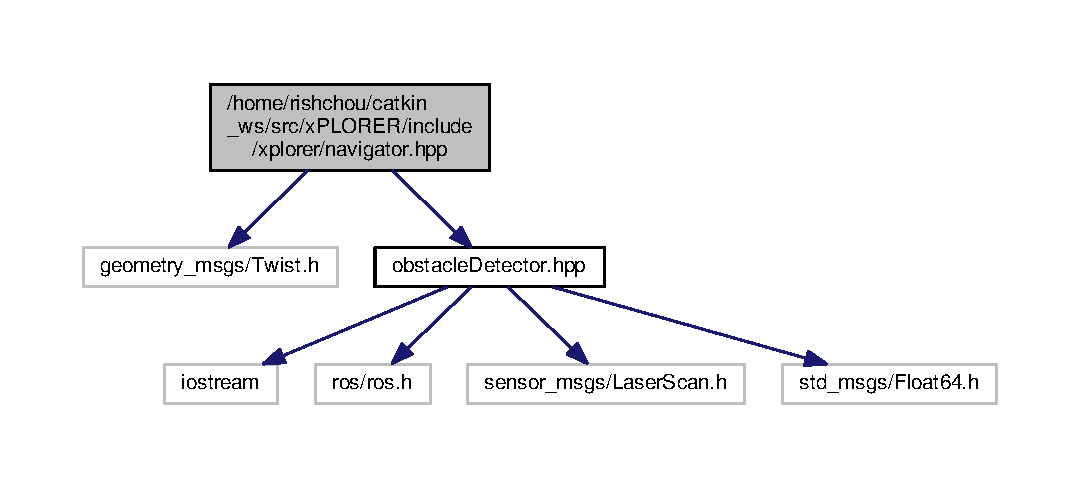
\includegraphics[width=350pt]{navigator_8hpp__incl}
\end{center}
\end{figure}
This graph shows which files directly or indirectly include this file\+:
\nopagebreak
\begin{figure}[H]
\begin{center}
\leavevmode
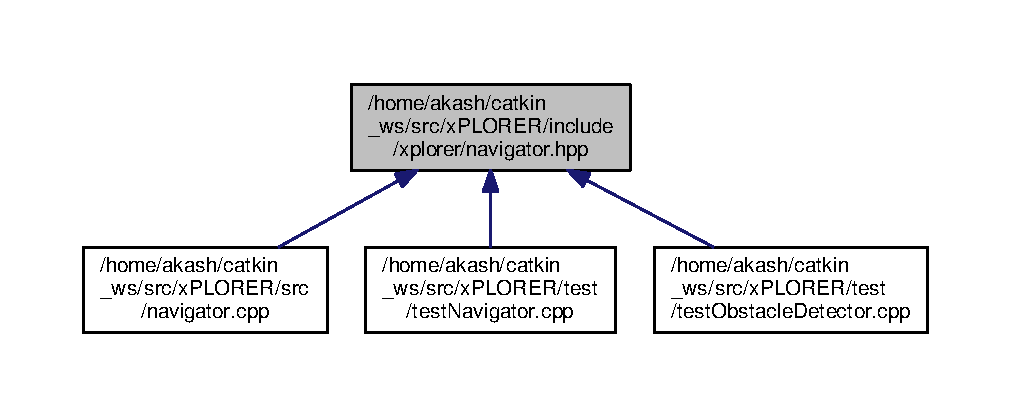
\includegraphics[width=350pt]{navigator_8hpp__dep__incl}
\end{center}
\end{figure}
\subsection*{Classes}
\begin{DoxyCompactItemize}
\item 
class \hyperlink{classnavigator}{navigator}
\begin{DoxyCompactList}\small\item\em Class for navigation part of the robot. \end{DoxyCompactList}\end{DoxyCompactItemize}


\subsection{Detailed Description}
\subsection*{\+: Class implementation for Robot Navigation functionality }

============================================================================

\begin{DoxyAuthor}{Author}
\+: Akash Atharv, Rishabh Choudhary 
\end{DoxyAuthor}
\begin{DoxyVersion}{Version}
\+: 1.\+0  \+: 3-\/\+Clause B\+SD Copyright (c) 2018, Akash Atharv, Rishabh Choudhary
\end{DoxyVersion}
Redistribution and use in source and binary forms, with or without modification, are permitted provided that the following conditions are met\+:


\begin{DoxyEnumerate}
\item Redistributions of source code must retain the above copyright notice, this list of conditions and the following disclaimer.
\item Redistributions in binary form must reproduce the above copyright notice, this list of conditions and the following disclaimer in the documentation and/or other materials provided with the distribution.
\item Neither the name of the copyright holder nor the names of its contributors may be used to endorse or promote products derived from this software without specific prior written permission.
\end{DoxyEnumerate}

T\+H\+IS S\+O\+F\+T\+W\+A\+RE IS P\+R\+O\+V\+I\+D\+ED BY T\+HE C\+O\+P\+Y\+R\+I\+G\+HT H\+O\+L\+D\+E\+RS A\+ND C\+O\+N\+T\+R\+I\+B\+U\+T\+O\+RS \char`\"{}\+A\+S 
\+I\+S\char`\"{} A\+ND A\+NY E\+X\+P\+R\+E\+SS OR I\+M\+P\+L\+I\+ED W\+A\+R\+R\+A\+N\+T\+I\+ES, I\+N\+C\+L\+U\+D\+I\+NG, B\+UT N\+OT L\+I\+M\+I\+T\+ED TO, T\+HE I\+M\+P\+L\+I\+ED W\+A\+R\+R\+A\+N\+T\+I\+ES OF M\+E\+R\+C\+H\+A\+N\+T\+A\+B\+I\+L\+I\+TY A\+ND F\+I\+T\+N\+E\+SS F\+OR A P\+A\+R\+T\+I\+C\+U\+L\+AR P\+U\+R\+P\+O\+SE A\+RE D\+I\+S\+C\+L\+A\+I\+M\+ED. IN NO E\+V\+E\+NT S\+H\+A\+LL T\+HE C\+O\+P\+Y\+R\+I\+G\+HT H\+O\+L\+D\+ER OR C\+O\+N\+T\+R\+I\+B\+U\+T\+O\+RS BE L\+I\+A\+B\+LE F\+OR A\+NY D\+I\+R\+E\+CT, I\+N\+D\+I\+R\+E\+CT, I\+N\+C\+I\+D\+E\+N\+T\+AL, S\+P\+E\+C\+I\+AL, E\+X\+E\+M\+P\+L\+A\+RY, OR C\+O\+N\+S\+E\+Q\+U\+E\+N\+T\+I\+AL D\+A\+M\+A\+G\+ES (I\+N\+C\+L\+U\+D\+I\+NG, B\+UT N\+OT L\+I\+M\+I\+T\+ED TO, P\+R\+O\+C\+U\+R\+E\+M\+E\+NT OF S\+U\+B\+S\+T\+I\+T\+U\+TE G\+O\+O\+DS OR S\+E\+R\+V\+I\+C\+ES; L\+O\+SS OF U\+SE, D\+A\+TA, OR P\+R\+O\+F\+I\+TS; OR B\+U\+S\+I\+N\+E\+SS I\+N\+T\+E\+R\+R\+U\+P\+T\+I\+ON) H\+O\+W\+E\+V\+ER C\+A\+U\+S\+ED A\+ND ON A\+NY T\+H\+E\+O\+RY OF L\+I\+A\+B\+I\+L\+I\+TY, W\+H\+E\+T\+H\+ER IN C\+O\+N\+T\+R\+A\+CT, S\+T\+R\+I\+CT L\+I\+A\+B\+I\+L\+I\+TY, OR T\+O\+RT (I\+N\+C\+L\+U\+D\+I\+NG N\+E\+G\+L\+I\+G\+E\+N\+CE OR O\+T\+H\+E\+R\+W\+I\+SE) A\+R\+I\+S\+I\+NG IN A\+NY W\+AY O\+UT OF T\+HE U\+SE OF T\+H\+IS S\+O\+F\+T\+W\+A\+RE, E\+V\+EN IF A\+D\+V\+I\+S\+ED OF T\+HE P\+O\+S\+S\+I\+B\+I\+L\+I\+TY OF S\+U\+CH D\+A\+M\+A\+GE. 
\hypertarget{obstacleDetector_8hpp}{}\section{/home/rishchou/catkin\+\_\+ws/src/x\+P\+L\+O\+R\+E\+R/include/xplorer/obstacle\+Detector.hpp File Reference}
\label{obstacleDetector_8hpp}\index{/home/rishchou/catkin\+\_\+ws/src/x\+P\+L\+O\+R\+E\+R/include/xplorer/obstacle\+Detector.\+hpp@{/home/rishchou/catkin\+\_\+ws/src/x\+P\+L\+O\+R\+E\+R/include/xplorer/obstacle\+Detector.\+hpp}}


\subsection*{\+: Class implementation for obstacle detection functionality } 


{\ttfamily \#include $<$iostream$>$}\\*
{\ttfamily \#include \char`\"{}ros/ros.\+h\char`\"{}}\\*
{\ttfamily \#include \char`\"{}sensor\+\_\+msgs/\+Laser\+Scan.\+h\char`\"{}}\\*
{\ttfamily \#include \char`\"{}std\+\_\+msgs/\+Float64.\+h\char`\"{}}\\*
Include dependency graph for obstacle\+Detector.\+hpp\+:
\nopagebreak
\begin{figure}[H]
\begin{center}
\leavevmode
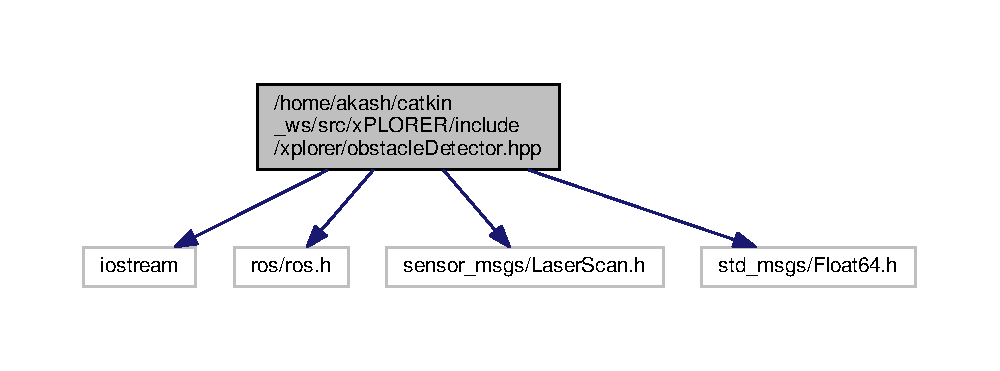
\includegraphics[width=350pt]{obstacleDetector_8hpp__incl}
\end{center}
\end{figure}
This graph shows which files directly or indirectly include this file\+:
\nopagebreak
\begin{figure}[H]
\begin{center}
\leavevmode
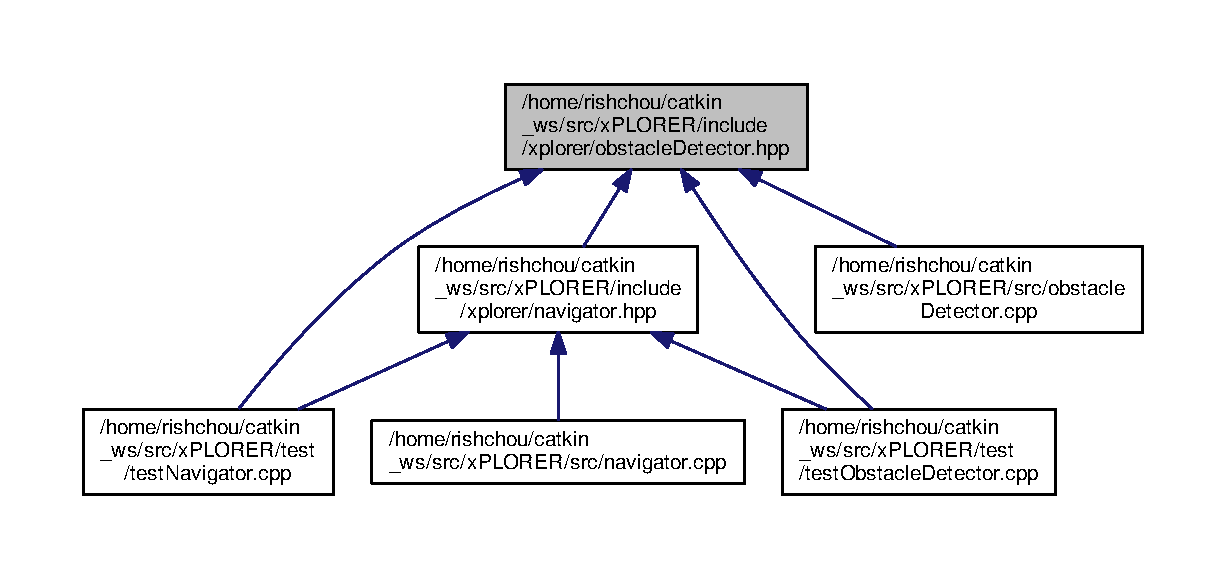
\includegraphics[width=350pt]{obstacleDetector_8hpp__dep__incl}
\end{center}
\end{figure}
\subsection*{Classes}
\begin{DoxyCompactItemize}
\item 
class \hyperlink{classobstacleDetector}{obstacle\+Detector}
\begin{DoxyCompactList}\small\item\em Class for obstacle\+Detection part of the robot. \end{DoxyCompactList}\end{DoxyCompactItemize}


\subsection{Detailed Description}
\subsection*{\+: Class implementation for obstacle detection functionality }

============================================================================

\begin{DoxyAuthor}{Author}
\+: Akash Atharv, Rishabh Choudhary 
\end{DoxyAuthor}
\begin{DoxyVersion}{Version}
\+: 1.\+0  \+: 3-\/\+Clause B\+SD Copyright (c) 2018, Akash Atharv, Rishabh Choudhary
\end{DoxyVersion}
Redistribution and use in source and binary forms, with or without modification, are permitted provided that the following conditions are met\+:


\begin{DoxyEnumerate}
\item Redistributions of source code must retain the above copyright notice, this list of conditions and the following disclaimer.
\item Redistributions in binary form must reproduce the above copyright notice, this list of conditions and the following disclaimer in the documentation and/or other materials provided with the distribution.
\item Neither the name of the copyright holder nor the names of its contributors may be used to endorse or promote products derived from this software without specific prior written permission.
\end{DoxyEnumerate}

T\+H\+IS S\+O\+F\+T\+W\+A\+RE IS P\+R\+O\+V\+I\+D\+ED BY T\+HE C\+O\+P\+Y\+R\+I\+G\+HT H\+O\+L\+D\+E\+RS A\+ND C\+O\+N\+T\+R\+I\+B\+U\+T\+O\+RS \char`\"{}\+A\+S 
\+I\+S\char`\"{} A\+ND A\+NY E\+X\+P\+R\+E\+SS OR I\+M\+P\+L\+I\+ED W\+A\+R\+R\+A\+N\+T\+I\+ES, I\+N\+C\+L\+U\+D\+I\+NG, B\+UT N\+OT L\+I\+M\+I\+T\+ED TO, T\+HE I\+M\+P\+L\+I\+ED W\+A\+R\+R\+A\+N\+T\+I\+ES OF M\+E\+R\+C\+H\+A\+N\+T\+A\+B\+I\+L\+I\+TY A\+ND F\+I\+T\+N\+E\+SS F\+OR A P\+A\+R\+T\+I\+C\+U\+L\+AR P\+U\+R\+P\+O\+SE A\+RE D\+I\+S\+C\+L\+A\+I\+M\+ED. IN NO E\+V\+E\+NT S\+H\+A\+LL T\+HE C\+O\+P\+Y\+R\+I\+G\+HT H\+O\+L\+D\+ER OR C\+O\+N\+T\+R\+I\+B\+U\+T\+O\+RS BE L\+I\+A\+B\+LE F\+OR A\+NY D\+I\+R\+E\+CT, I\+N\+D\+I\+R\+E\+CT, I\+N\+C\+I\+D\+E\+N\+T\+AL, S\+P\+E\+C\+I\+AL, E\+X\+E\+M\+P\+L\+A\+RY, OR C\+O\+N\+S\+E\+Q\+U\+E\+N\+T\+I\+AL D\+A\+M\+A\+G\+ES (I\+N\+C\+L\+U\+D\+I\+NG, B\+UT N\+OT L\+I\+M\+I\+T\+ED TO, P\+R\+O\+C\+U\+R\+E\+M\+E\+NT OF S\+U\+B\+S\+T\+I\+T\+U\+TE G\+O\+O\+DS OR S\+E\+R\+V\+I\+C\+ES; L\+O\+SS OF U\+SE, D\+A\+TA, OR P\+R\+O\+F\+I\+TS; OR B\+U\+S\+I\+N\+E\+SS I\+N\+T\+E\+R\+R\+U\+P\+T\+I\+ON) H\+O\+W\+E\+V\+ER C\+A\+U\+S\+ED A\+ND ON A\+NY T\+H\+E\+O\+RY OF L\+I\+A\+B\+I\+L\+I\+TY, W\+H\+E\+T\+H\+ER IN C\+O\+N\+T\+R\+A\+CT, S\+T\+R\+I\+CT L\+I\+A\+B\+I\+L\+I\+TY, OR T\+O\+RT (I\+N\+C\+L\+U\+D\+I\+NG N\+E\+G\+L\+I\+G\+E\+N\+CE OR O\+T\+H\+E\+R\+W\+I\+SE) A\+R\+I\+S\+I\+NG IN A\+NY W\+AY O\+UT OF T\+HE U\+SE OF T\+H\+IS S\+O\+F\+T\+W\+A\+RE, E\+V\+EN IF A\+D\+V\+I\+S\+ED OF T\+HE P\+O\+S\+S\+I\+B\+I\+L\+I\+TY OF S\+U\+CH D\+A\+M\+A\+GE. 
\hypertarget{navigator_8cpp}{}\section{/home/rishchou/catkin\+\_\+ws/src/x\+P\+L\+O\+R\+E\+R/src/navigator.cpp File Reference}
\label{navigator_8cpp}\index{/home/rishchou/catkin\+\_\+ws/src/x\+P\+L\+O\+R\+E\+R/src/navigator.\+cpp@{/home/rishchou/catkin\+\_\+ws/src/x\+P\+L\+O\+R\+E\+R/src/navigator.\+cpp}}


\subsection*{\+: Functional implementation for Robot Navigation functionality } 


{\ttfamily \#include \char`\"{}../include/xplorer/navigator.\+hpp\char`\"{}}\\*
Include dependency graph for navigator.\+cpp\+:
\nopagebreak
\begin{figure}[H]
\begin{center}
\leavevmode
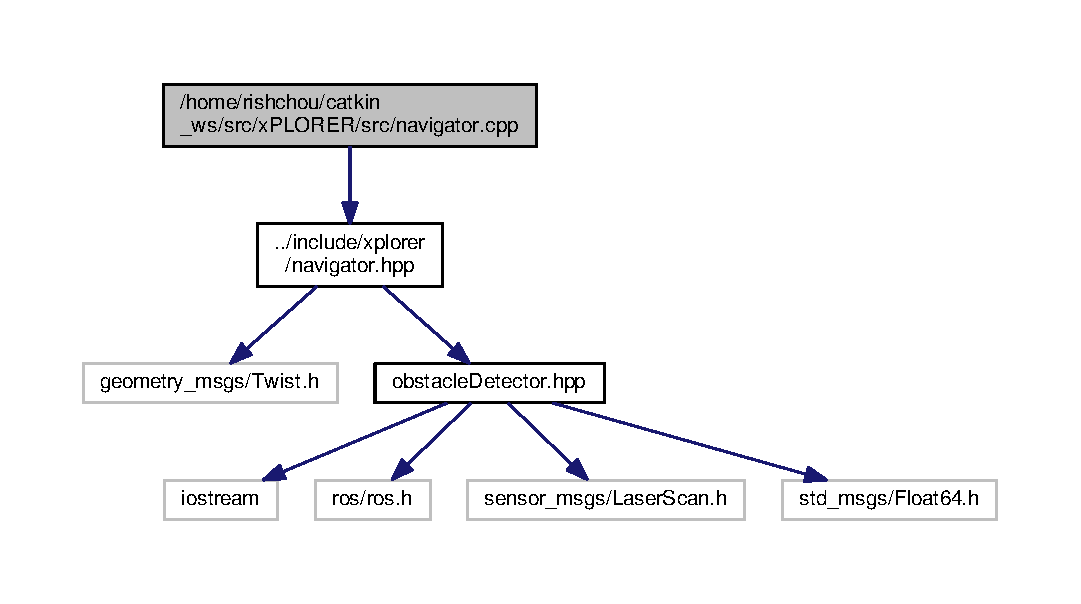
\includegraphics[width=350pt]{navigator_8cpp__incl}
\end{center}
\end{figure}


\subsection{Detailed Description}
\subsection*{\+: Functional implementation for Robot Navigation functionality }

============================================================================

\begin{DoxyAuthor}{Author}
\+: Akash Atharv, Rishabh Choudhary 
\end{DoxyAuthor}
\begin{DoxyVersion}{Version}
\+: 1.\+0  \+: 3-\/\+Clause B\+SD Copyright (c) 2018, Akash Atharv, Rishabh Choudhary
\end{DoxyVersion}
Redistribution and use in source and binary forms, with or without modification, are permitted provided that the following conditions are met\+:


\begin{DoxyEnumerate}
\item Redistributions of source code must retain the above copyright notice, this list of conditions and the following disclaimer.
\item Redistributions in binary form must reproduce the above copyright notice, this list of conditions and the following disclaimer in the documentation and/or other materials provided with the distribution.
\item Neither the name of the copyright holder nor the names of its contributors may be used to endorse or promote products derived from this software without specific prior written permission.
\end{DoxyEnumerate}

T\+H\+IS S\+O\+F\+T\+W\+A\+RE IS P\+R\+O\+V\+I\+D\+ED BY T\+HE C\+O\+P\+Y\+R\+I\+G\+HT H\+O\+L\+D\+E\+RS A\+ND C\+O\+N\+T\+R\+I\+B\+U\+T\+O\+RS \char`\"{}\+A\+S 
\+I\+S\char`\"{} A\+ND A\+NY E\+X\+P\+R\+E\+SS OR I\+M\+P\+L\+I\+ED W\+A\+R\+R\+A\+N\+T\+I\+ES, I\+N\+C\+L\+U\+D\+I\+NG, B\+UT N\+OT L\+I\+M\+I\+T\+ED TO, T\+HE I\+M\+P\+L\+I\+ED W\+A\+R\+R\+A\+N\+T\+I\+ES OF M\+E\+R\+C\+H\+A\+N\+T\+A\+B\+I\+L\+I\+TY A\+ND F\+I\+T\+N\+E\+SS F\+OR A P\+A\+R\+T\+I\+C\+U\+L\+AR P\+U\+R\+P\+O\+SE A\+RE D\+I\+S\+C\+L\+A\+I\+M\+ED. IN NO E\+V\+E\+NT S\+H\+A\+LL T\+HE C\+O\+P\+Y\+R\+I\+G\+HT H\+O\+L\+D\+ER OR C\+O\+N\+T\+R\+I\+B\+U\+T\+O\+RS BE L\+I\+A\+B\+LE F\+OR A\+NY D\+I\+R\+E\+CT, I\+N\+D\+I\+R\+E\+CT, I\+N\+C\+I\+D\+E\+N\+T\+AL, S\+P\+E\+C\+I\+AL, E\+X\+E\+M\+P\+L\+A\+RY, OR C\+O\+N\+S\+E\+Q\+U\+E\+N\+T\+I\+AL D\+A\+M\+A\+G\+ES (I\+N\+C\+L\+U\+D\+I\+NG, B\+UT N\+OT L\+I\+M\+I\+T\+ED TO, P\+R\+O\+C\+U\+R\+E\+M\+E\+NT OF S\+U\+B\+S\+T\+I\+T\+U\+TE G\+O\+O\+DS OR S\+E\+R\+V\+I\+C\+ES; L\+O\+SS OF U\+SE, D\+A\+TA, OR P\+R\+O\+F\+I\+TS; OR B\+U\+S\+I\+N\+E\+SS I\+N\+T\+E\+R\+R\+U\+P\+T\+I\+ON) H\+O\+W\+E\+V\+ER C\+A\+U\+S\+ED A\+ND ON A\+NY T\+H\+E\+O\+RY OF L\+I\+A\+B\+I\+L\+I\+TY, W\+H\+E\+T\+H\+ER IN C\+O\+N\+T\+R\+A\+CT, S\+T\+R\+I\+CT L\+I\+A\+B\+I\+L\+I\+TY, OR T\+O\+RT (I\+N\+C\+L\+U\+D\+I\+NG N\+E\+G\+L\+I\+G\+E\+N\+CE OR O\+T\+H\+E\+R\+W\+I\+SE) A\+R\+I\+S\+I\+NG IN A\+NY W\+AY O\+UT OF T\+HE U\+SE OF T\+H\+IS S\+O\+F\+T\+W\+A\+RE, E\+V\+EN IF A\+D\+V\+I\+S\+ED OF T\+HE P\+O\+S\+S\+I\+B\+I\+L\+I\+TY OF S\+U\+CH D\+A\+M\+A\+GE. 
\hypertarget{obstacleDetector_8cpp}{}\section{/home/rishchou/catkin\+\_\+ws/src/x\+P\+L\+O\+R\+E\+R/src/obstacle\+Detector.cpp File Reference}
\label{obstacleDetector_8cpp}\index{/home/rishchou/catkin\+\_\+ws/src/x\+P\+L\+O\+R\+E\+R/src/obstacle\+Detector.\+cpp@{/home/rishchou/catkin\+\_\+ws/src/x\+P\+L\+O\+R\+E\+R/src/obstacle\+Detector.\+cpp}}


\subsection*{\+: Functional implementation for obstacle detection functionality } 


{\ttfamily \#include \char`\"{}../include/xplorer/obstacle\+Detector.\+hpp\char`\"{}}\\*
Include dependency graph for obstacle\+Detector.\+cpp\+:
\nopagebreak
\begin{figure}[H]
\begin{center}
\leavevmode
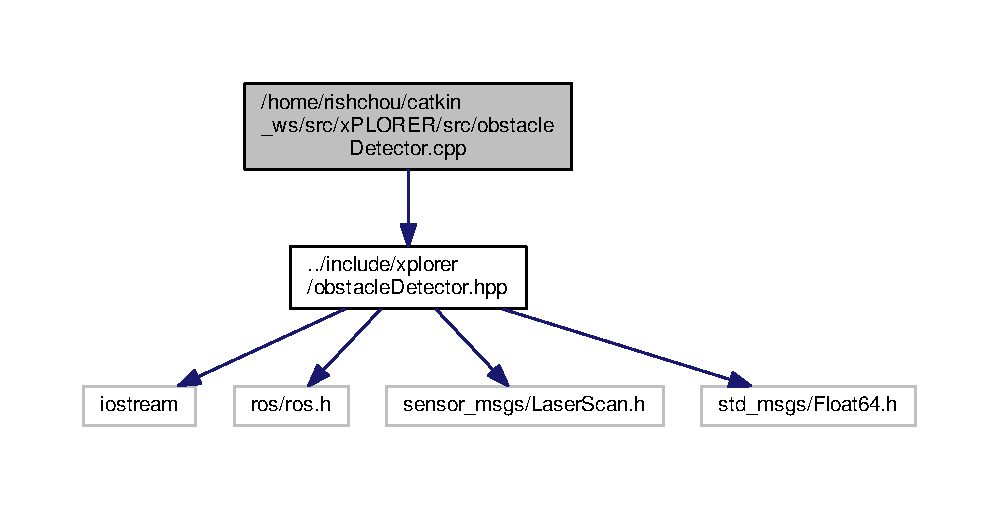
\includegraphics[width=350pt]{obstacleDetector_8cpp__incl}
\end{center}
\end{figure}


\subsection{Detailed Description}
\subsection*{\+: Functional implementation for obstacle detection functionality }

============================================================================

\begin{DoxyAuthor}{Author}
\+: Akash Atharv, Rishabh Choudhary 
\end{DoxyAuthor}
\begin{DoxyVersion}{Version}
\+: 1.\+0  \+: 3-\/\+Clause B\+SD
\end{DoxyVersion}
Copyright (c) 2018, Akash Atharv, Rishabh Choudhary

Redistribution and use in source and binary forms, with or without modification, are permitted provided that the following conditions are met\+:


\begin{DoxyEnumerate}
\item Redistributions of source code must retain the above copyright notice, this list of conditions and the following disclaimer.
\item Redistributions in binary form must reproduce the above copyright notice, this list of conditions and the following disclaimer in the documentation and/or other materials provided with the distribution.
\item Neither the name of the copyright holder nor the names of its contributors may be used to endorse or promote products derived from this software without specific prior written permission.
\end{DoxyEnumerate}

T\+H\+IS S\+O\+F\+T\+W\+A\+RE IS P\+R\+O\+V\+I\+D\+ED BY T\+HE C\+O\+P\+Y\+R\+I\+G\+HT H\+O\+L\+D\+E\+RS A\+ND C\+O\+N\+T\+R\+I\+B\+U\+T\+O\+RS \char`\"{}\+A\+S 
\+I\+S\char`\"{} A\+ND A\+NY E\+X\+P\+R\+E\+SS OR I\+M\+P\+L\+I\+ED W\+A\+R\+R\+A\+N\+T\+I\+ES, I\+N\+C\+L\+U\+D\+I\+NG, B\+UT N\+OT L\+I\+M\+I\+T\+ED TO, T\+HE I\+M\+P\+L\+I\+ED W\+A\+R\+R\+A\+N\+T\+I\+ES OF M\+E\+R\+C\+H\+A\+N\+T\+A\+B\+I\+L\+I\+TY A\+ND F\+I\+T\+N\+E\+SS F\+OR A P\+A\+R\+T\+I\+C\+U\+L\+AR P\+U\+R\+P\+O\+SE A\+RE D\+I\+S\+C\+L\+A\+I\+M\+ED. IN NO E\+V\+E\+NT S\+H\+A\+LL T\+HE C\+O\+P\+Y\+R\+I\+G\+HT H\+O\+L\+D\+ER OR C\+O\+N\+T\+R\+I\+B\+U\+T\+O\+RS BE L\+I\+A\+B\+LE F\+OR A\+NY D\+I\+R\+E\+CT, I\+N\+D\+I\+R\+E\+CT, I\+N\+C\+I\+D\+E\+N\+T\+AL, S\+P\+E\+C\+I\+AL, E\+X\+E\+M\+P\+L\+A\+RY, OR C\+O\+N\+S\+E\+Q\+U\+E\+N\+T\+I\+AL D\+A\+M\+A\+G\+ES (I\+N\+C\+L\+U\+D\+I\+NG, B\+UT N\+OT L\+I\+M\+I\+T\+ED TO, P\+R\+O\+C\+U\+R\+E\+M\+E\+NT OF S\+U\+B\+S\+T\+I\+T\+U\+TE G\+O\+O\+DS OR S\+E\+R\+V\+I\+C\+ES; L\+O\+SS OF U\+SE, D\+A\+TA, OR P\+R\+O\+F\+I\+TS; OR B\+U\+S\+I\+N\+E\+SS I\+N\+T\+E\+R\+R\+U\+P\+T\+I\+ON) H\+O\+W\+E\+V\+ER C\+A\+U\+S\+ED A\+ND ON A\+NY T\+H\+E\+O\+RY OF L\+I\+A\+B\+I\+L\+I\+TY, W\+H\+E\+T\+H\+ER IN C\+O\+N\+T\+R\+A\+CT, S\+T\+R\+I\+CT L\+I\+A\+B\+I\+L\+I\+TY, OR T\+O\+RT (I\+N\+C\+L\+U\+D\+I\+NG N\+E\+G\+L\+I\+G\+E\+N\+CE OR O\+T\+H\+E\+R\+W\+I\+SE) A\+R\+I\+S\+I\+NG IN A\+NY W\+AY O\+UT OF T\+HE U\+SE OF T\+H\+IS S\+O\+F\+T\+W\+A\+RE, E\+V\+EN IF A\+D\+V\+I\+S\+ED OF T\+HE P\+O\+S\+S\+I\+B\+I\+L\+I\+TY OF S\+U\+CH D\+A\+M\+A\+GE. 
\hypertarget{testNavigator_8cpp}{}\section{/home/akash/catkin\+\_\+ws/src/x\+P\+L\+O\+R\+E\+R/test/test\+Navigator.cpp File Reference}
\label{testNavigator_8cpp}\index{/home/akash/catkin\+\_\+ws/src/x\+P\+L\+O\+R\+E\+R/test/test\+Navigator.\+cpp@{/home/akash/catkin\+\_\+ws/src/x\+P\+L\+O\+R\+E\+R/test/test\+Navigator.\+cpp}}


\subsection*{\+: Test file for testing class Navigator } 


{\ttfamily \#include $<$ros/ros.\+h$>$}\\*
{\ttfamily \#include $<$gtest/gtest.\+h$>$}\\*
{\ttfamily \#include \char`\"{}../include/xplorer/obstacle\+Detector.\+hpp\char`\"{}}\\*
{\ttfamily \#include \char`\"{}../include/xplorer/navigator.\+hpp\char`\"{}}\\*
Include dependency graph for test\+Navigator.\+cpp\+:
\nopagebreak
\begin{figure}[H]
\begin{center}
\leavevmode
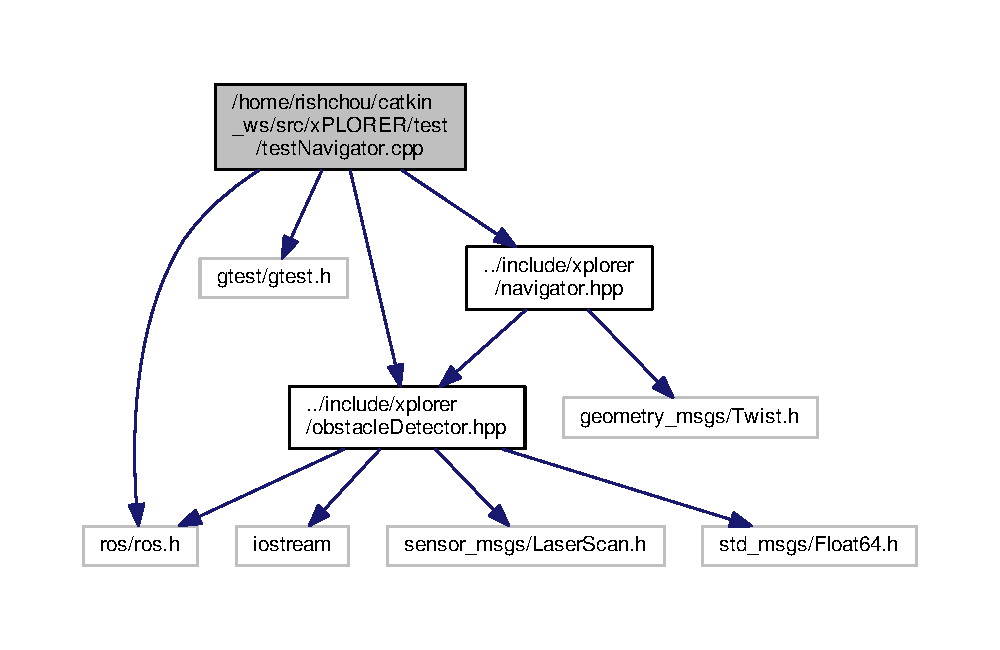
\includegraphics[width=350pt]{testNavigator_8cpp__incl}
\end{center}
\end{figure}
\subsection*{Classes}
\begin{DoxyCompactItemize}
\item 
class \hyperlink{classTestClass}{Test\+Class}
\begin{DoxyCompactList}\small\item\em Class for testing. \end{DoxyCompactList}\end{DoxyCompactItemize}
\subsection*{Functions}
\begin{DoxyCompactItemize}
\item 
\hyperlink{testNavigator_8cpp_aaa6d5c559f5ac48e4423417c763ac8ca}{T\+E\+ST} (Navigator\+Component\+Test, Navigator\+\_\+\+Object\+\_\+is\+\_\+initialized)
\begin{DoxyCompactList}\small\item\em Test to find if object is initialized and the navigator program functions properly. \end{DoxyCompactList}\item 
\hyperlink{testNavigator_8cpp_a5a3668d78e02d65d8c265ac6503eda58}{T\+E\+ST} (Navigator\+Component\+Test, Navigator\+Publisher\+Test)
\begin{DoxyCompactList}\small\item\em Test to find if publisher for /mobile\+\_\+base/commands/velocity is working. \end{DoxyCompactList}\item 
\hyperlink{testNavigator_8cpp_a87601526f6eb07bcd540b0c8604e776a}{T\+E\+ST} (Navigator\+Component\+Test, Navigator\+Subscriber\+Test)
\begin{DoxyCompactList}\small\item\em Test to find if subscriber for /dist is working. \end{DoxyCompactList}\item 
\hyperlink{testNavigator_8cpp_a5e7522796d7b492cf2d71a2e093801cd}{T\+E\+ST} (Navigator\+Component\+Test, Robot\+Navigator\+Test)
\begin{DoxyCompactList}\small\item\em Test to find if the main function for robot movement is working. \end{DoxyCompactList}\end{DoxyCompactItemize}


\subsection{Detailed Description}
\subsection*{\+: Test file for testing class Navigator }

============================================================================

\begin{DoxyAuthor}{Author}
\+: Akash Atharv, Rishabh Choudhary 
\end{DoxyAuthor}
\begin{DoxyVersion}{Version}
\+: 1.\+0  \+: 3-\/\+Clause B\+SD Copyright (c) 2018, Akash Atharv, Rishabh Choudhary
\end{DoxyVersion}
Redistribution and use in source and binary forms, with or without modification, are permitted provided that the following conditions are met\+:


\begin{DoxyEnumerate}
\item Redistributions of source code must retain the above copyright notice, this list of conditions and the following disclaimer.
\item Redistributions in binary form must reproduce the above copyright notice, this list of conditions and the following disclaimer in the documentation and/or other materials provided with the distribution.
\item Neither the name of the copyright holder nor the names of its contributors may be used to endorse or promote products derived from this software without specific prior written permission.
\end{DoxyEnumerate}

T\+H\+IS S\+O\+F\+T\+W\+A\+RE IS P\+R\+O\+V\+I\+D\+ED BY T\+HE C\+O\+P\+Y\+R\+I\+G\+HT H\+O\+L\+D\+E\+RS A\+ND C\+O\+N\+T\+R\+I\+B\+U\+T\+O\+RS \char`\"{}\+A\+S 
\+I\+S\char`\"{} A\+ND A\+NY E\+X\+P\+R\+E\+SS OR I\+M\+P\+L\+I\+ED W\+A\+R\+R\+A\+N\+T\+I\+ES, I\+N\+C\+L\+U\+D\+I\+NG, B\+UT N\+OT L\+I\+M\+I\+T\+ED TO, T\+HE I\+M\+P\+L\+I\+ED W\+A\+R\+R\+A\+N\+T\+I\+ES OF M\+E\+R\+C\+H\+A\+N\+T\+A\+B\+I\+L\+I\+TY A\+ND F\+I\+T\+N\+E\+SS F\+OR A P\+A\+R\+T\+I\+C\+U\+L\+AR P\+U\+R\+P\+O\+SE A\+RE D\+I\+S\+C\+L\+A\+I\+M\+ED. IN NO E\+V\+E\+NT S\+H\+A\+LL T\+HE C\+O\+P\+Y\+R\+I\+G\+HT H\+O\+L\+D\+ER OR C\+O\+N\+T\+R\+I\+B\+U\+T\+O\+RS BE L\+I\+A\+B\+LE F\+OR A\+NY D\+I\+R\+E\+CT, I\+N\+D\+I\+R\+E\+CT, I\+N\+C\+I\+D\+E\+N\+T\+AL, S\+P\+E\+C\+I\+AL, E\+X\+E\+M\+P\+L\+A\+RY, OR C\+O\+N\+S\+E\+Q\+U\+E\+N\+T\+I\+AL D\+A\+M\+A\+G\+ES (I\+N\+C\+L\+U\+D\+I\+NG, B\+UT N\+OT L\+I\+M\+I\+T\+ED TO, P\+R\+O\+C\+U\+R\+E\+M\+E\+NT OF S\+U\+B\+S\+T\+I\+T\+U\+TE G\+O\+O\+DS OR S\+E\+R\+V\+I\+C\+ES; L\+O\+SS OF U\+SE, D\+A\+TA, OR P\+R\+O\+F\+I\+TS; OR B\+U\+S\+I\+N\+E\+SS I\+N\+T\+E\+R\+R\+U\+P\+T\+I\+ON) H\+O\+W\+E\+V\+ER C\+A\+U\+S\+ED A\+ND ON A\+NY T\+H\+E\+O\+RY OF L\+I\+A\+B\+I\+L\+I\+TY, W\+H\+E\+T\+H\+ER IN C\+O\+N\+T\+R\+A\+CT, S\+T\+R\+I\+CT L\+I\+A\+B\+I\+L\+I\+TY, OR T\+O\+RT (I\+N\+C\+L\+U\+D\+I\+NG N\+E\+G\+L\+I\+G\+E\+N\+CE OR O\+T\+H\+E\+R\+W\+I\+SE) A\+R\+I\+S\+I\+NG IN A\+NY W\+AY O\+UT OF T\+HE U\+SE OF T\+H\+IS S\+O\+F\+T\+W\+A\+RE, E\+V\+EN IF A\+D\+V\+I\+S\+ED OF T\+HE P\+O\+S\+S\+I\+B\+I\+L\+I\+TY OF S\+U\+CH D\+A\+M\+A\+GE. 

\subsection{Function Documentation}
\index{test\+Navigator.\+cpp@{test\+Navigator.\+cpp}!T\+E\+ST@{T\+E\+ST}}
\index{T\+E\+ST@{T\+E\+ST}!test\+Navigator.\+cpp@{test\+Navigator.\+cpp}}
\subsubsection[{\texorpdfstring{T\+E\+S\+T(\+Navigator\+Component\+Test, Navigator\+\_\+\+Object\+\_\+is\+\_\+initialized)}{TEST(NavigatorComponentTest, Navigator_Object_is_initialized)}}]{\setlength{\rightskip}{0pt plus 5cm}T\+E\+ST (
\begin{DoxyParamCaption}
\item[{Navigator\+Component\+Test}]{, }
\item[{Navigator\+\_\+\+Object\+\_\+is\+\_\+initialized}]{}
\end{DoxyParamCaption}
)}\hypertarget{testNavigator_8cpp_aaa6d5c559f5ac48e4423417c763ac8ca}{}\label{testNavigator_8cpp_aaa6d5c559f5ac48e4423417c763ac8ca}


Test to find if object is initialized and the navigator program functions properly. 


\begin{DoxyParams}{Parameters}
{\em Navigator\+Component\+Test} & Gtest framework \\
\hline
{\em Navigator\+\_\+\+Object\+\_\+is\+\_\+initialized} & Test name \\
\hline
\end{DoxyParams}
\index{test\+Navigator.\+cpp@{test\+Navigator.\+cpp}!T\+E\+ST@{T\+E\+ST}}
\index{T\+E\+ST@{T\+E\+ST}!test\+Navigator.\+cpp@{test\+Navigator.\+cpp}}
\subsubsection[{\texorpdfstring{T\+E\+S\+T(\+Navigator\+Component\+Test, Navigator\+Publisher\+Test)}{TEST(NavigatorComponentTest, NavigatorPublisherTest)}}]{\setlength{\rightskip}{0pt plus 5cm}T\+E\+ST (
\begin{DoxyParamCaption}
\item[{Navigator\+Component\+Test}]{, }
\item[{Navigator\+Publisher\+Test}]{}
\end{DoxyParamCaption}
)}\hypertarget{testNavigator_8cpp_a5a3668d78e02d65d8c265ac6503eda58}{}\label{testNavigator_8cpp_a5a3668d78e02d65d8c265ac6503eda58}


Test to find if publisher for /mobile\+\_\+base/commands/velocity is working. 


\begin{DoxyParams}{Parameters}
{\em Navigator\+Component\+Test} & Gtest framework \\
\hline
{\em Publish\+\_\+\+Test} & Test name \\
\hline
\end{DoxyParams}
\index{test\+Navigator.\+cpp@{test\+Navigator.\+cpp}!T\+E\+ST@{T\+E\+ST}}
\index{T\+E\+ST@{T\+E\+ST}!test\+Navigator.\+cpp@{test\+Navigator.\+cpp}}
\subsubsection[{\texorpdfstring{T\+E\+S\+T(\+Navigator\+Component\+Test, Navigator\+Subscriber\+Test)}{TEST(NavigatorComponentTest, NavigatorSubscriberTest)}}]{\setlength{\rightskip}{0pt plus 5cm}T\+E\+ST (
\begin{DoxyParamCaption}
\item[{Navigator\+Component\+Test}]{, }
\item[{Navigator\+Subscriber\+Test}]{}
\end{DoxyParamCaption}
)}\hypertarget{testNavigator_8cpp_a87601526f6eb07bcd540b0c8604e776a}{}\label{testNavigator_8cpp_a87601526f6eb07bcd540b0c8604e776a}


Test to find if subscriber for /dist is working. 


\begin{DoxyParams}{Parameters}
{\em Navigator\+Component\+Test} & Gtest framework \\
\hline
{\em Subscribe\+\_\+\+Test} & Test name \\
\hline
\end{DoxyParams}
\index{test\+Navigator.\+cpp@{test\+Navigator.\+cpp}!T\+E\+ST@{T\+E\+ST}}
\index{T\+E\+ST@{T\+E\+ST}!test\+Navigator.\+cpp@{test\+Navigator.\+cpp}}
\subsubsection[{\texorpdfstring{T\+E\+S\+T(\+Navigator\+Component\+Test, Robot\+Navigator\+Test)}{TEST(NavigatorComponentTest, RobotNavigatorTest)}}]{\setlength{\rightskip}{0pt plus 5cm}T\+E\+ST (
\begin{DoxyParamCaption}
\item[{Navigator\+Component\+Test}]{, }
\item[{Robot\+Navigator\+Test}]{}
\end{DoxyParamCaption}
)}\hypertarget{testNavigator_8cpp_a5e7522796d7b492cf2d71a2e093801cd}{}\label{testNavigator_8cpp_a5e7522796d7b492cf2d71a2e093801cd}


Test to find if the main function for robot movement is working. 


\begin{DoxyParams}{Parameters}
{\em Navigator\+Component\+Test} & Gtest framework \\
\hline
{\em Robot\+Navigator\+Test} & Test name \\
\hline
\end{DoxyParams}

\hypertarget{testObstacleDetector_8cpp}{}\section{/home/rishchou/catkin\+\_\+ws/src/x\+P\+L\+O\+R\+E\+R/test/test\+Obstacle\+Detector.cpp File Reference}
\label{testObstacleDetector_8cpp}\index{/home/rishchou/catkin\+\_\+ws/src/x\+P\+L\+O\+R\+E\+R/test/test\+Obstacle\+Detector.\+cpp@{/home/rishchou/catkin\+\_\+ws/src/x\+P\+L\+O\+R\+E\+R/test/test\+Obstacle\+Detector.\+cpp}}


\subsection*{\+: Test file for testing class \hyperlink{classobstacleDetector}{obstacle\+Detector} } 


{\ttfamily \#include $<$ros/ros.\+h$>$}\\*
{\ttfamily \#include $<$gtest/gtest.\+h$>$}\\*
{\ttfamily \#include \char`\"{}../include/xplorer/obstacle\+Detector.\+hpp\char`\"{}}\\*
{\ttfamily \#include \char`\"{}../include/xplorer/navigator.\+hpp\char`\"{}}\\*
Include dependency graph for test\+Obstacle\+Detector.\+cpp\+:
\nopagebreak
\begin{figure}[H]
\begin{center}
\leavevmode
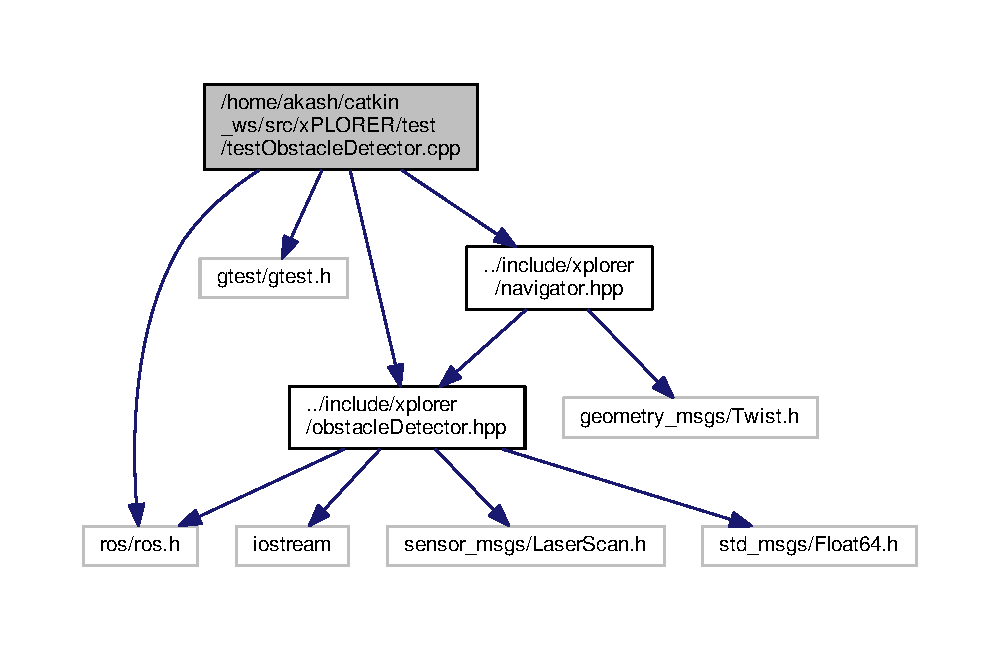
\includegraphics[width=350pt]{testObstacleDetector_8cpp__incl}
\end{center}
\end{figure}
\subsection*{Functions}
\begin{DoxyCompactItemize}
\item 
\hyperlink{testObstacleDetector_8cpp_a37b97005e72f34de8abedb5c5ade832a}{T\+E\+ST} (T\+E\+S\+T\+Suite, Obstacle\+Detector\+\_\+\+Object\+\_\+is\+\_\+initialized)
\begin{DoxyCompactList}\small\item\em Test to find if object is initialized and the \hyperlink{classobstacleDetector}{obstacle\+Detector} program functions properly. \end{DoxyCompactList}\item 
\hyperlink{testObstacleDetector_8cpp_a278e5d4795cf273fb11e60d147ad0f36}{T\+E\+ST} (T\+E\+S\+T\+Suite, Collision\+\_\+should\+\_\+not\+\_\+be\+\_\+detected)
\begin{DoxyCompactList}\small\item\em Test to find if collision is not detected at a particular time. \end{DoxyCompactList}\item 
\hyperlink{testObstacleDetector_8cpp_a49669a17f3daac997dcfaa2fd64a8337}{T\+E\+ST} (T\+E\+S\+T\+Suite, Collision\+\_\+should\+\_\+be\+\_\+detected)
\begin{DoxyCompactList}\small\item\em Test to find if collision is detected at a particular time. \end{DoxyCompactList}\end{DoxyCompactItemize}


\subsection{Detailed Description}
\subsection*{\+: Test file for testing class \hyperlink{classobstacleDetector}{obstacle\+Detector} }

============================================================================

\begin{DoxyAuthor}{Author}
\+: Akash Atharv, Rishabh Choudhary 
\end{DoxyAuthor}
\begin{DoxyVersion}{Version}
\+: 1.\+0  \+: 3-\/\+Clause B\+SD Copyright (c) 2018, Akash Atharv, Rishabh Choudhary
\end{DoxyVersion}
Redistribution and use in source and binary forms, with or without modification, are permitted provided that the following conditions are met\+:


\begin{DoxyEnumerate}
\item Redistributions of source code must retain the above copyright notice, this list of conditions and the following disclaimer.
\item Redistributions in binary form must reproduce the above copyright notice, this list of conditions and the following disclaimer in the documentation and/or other materials provided with the distribution.
\item Neither the name of the copyright holder nor the names of its contributors may be used to endorse or promote products derived from this software without specific prior written permission.
\end{DoxyEnumerate}

T\+H\+IS S\+O\+F\+T\+W\+A\+RE IS P\+R\+O\+V\+I\+D\+ED BY T\+HE C\+O\+P\+Y\+R\+I\+G\+HT H\+O\+L\+D\+E\+RS A\+ND C\+O\+N\+T\+R\+I\+B\+U\+T\+O\+RS \char`\"{}\+A\+S 
\+I\+S\char`\"{} A\+ND A\+NY E\+X\+P\+R\+E\+SS OR I\+M\+P\+L\+I\+ED W\+A\+R\+R\+A\+N\+T\+I\+ES, I\+N\+C\+L\+U\+D\+I\+NG, B\+UT N\+OT L\+I\+M\+I\+T\+ED TO, T\+HE I\+M\+P\+L\+I\+ED W\+A\+R\+R\+A\+N\+T\+I\+ES OF M\+E\+R\+C\+H\+A\+N\+T\+A\+B\+I\+L\+I\+TY A\+ND F\+I\+T\+N\+E\+SS F\+OR A P\+A\+R\+T\+I\+C\+U\+L\+AR P\+U\+R\+P\+O\+SE A\+RE D\+I\+S\+C\+L\+A\+I\+M\+ED. IN NO E\+V\+E\+NT S\+H\+A\+LL T\+HE C\+O\+P\+Y\+R\+I\+G\+HT H\+O\+L\+D\+ER OR C\+O\+N\+T\+R\+I\+B\+U\+T\+O\+RS BE L\+I\+A\+B\+LE F\+OR A\+NY D\+I\+R\+E\+CT, I\+N\+D\+I\+R\+E\+CT, I\+N\+C\+I\+D\+E\+N\+T\+AL, S\+P\+E\+C\+I\+AL, E\+X\+E\+M\+P\+L\+A\+RY, OR C\+O\+N\+S\+E\+Q\+U\+E\+N\+T\+I\+AL D\+A\+M\+A\+G\+ES (I\+N\+C\+L\+U\+D\+I\+NG, B\+UT N\+OT L\+I\+M\+I\+T\+ED TO, P\+R\+O\+C\+U\+R\+E\+M\+E\+NT OF S\+U\+B\+S\+T\+I\+T\+U\+TE G\+O\+O\+DS OR S\+E\+R\+V\+I\+C\+ES; L\+O\+SS OF U\+SE, D\+A\+TA, OR P\+R\+O\+F\+I\+TS; OR B\+U\+S\+I\+N\+E\+SS I\+N\+T\+E\+R\+R\+U\+P\+T\+I\+ON) H\+O\+W\+E\+V\+ER C\+A\+U\+S\+ED A\+ND ON A\+NY T\+H\+E\+O\+RY OF L\+I\+A\+B\+I\+L\+I\+TY, W\+H\+E\+T\+H\+ER IN C\+O\+N\+T\+R\+A\+CT, S\+T\+R\+I\+CT L\+I\+A\+B\+I\+L\+I\+TY, OR T\+O\+RT (I\+N\+C\+L\+U\+D\+I\+NG N\+E\+G\+L\+I\+G\+E\+N\+CE OR O\+T\+H\+E\+R\+W\+I\+SE) A\+R\+I\+S\+I\+NG IN A\+NY W\+AY O\+UT OF T\+HE U\+SE OF T\+H\+IS S\+O\+F\+T\+W\+A\+RE, E\+V\+EN IF A\+D\+V\+I\+S\+ED OF T\+HE P\+O\+S\+S\+I\+B\+I\+L\+I\+TY OF S\+U\+CH D\+A\+M\+A\+GE. 

\subsection{Function Documentation}
\index{test\+Obstacle\+Detector.\+cpp@{test\+Obstacle\+Detector.\+cpp}!T\+E\+ST@{T\+E\+ST}}
\index{T\+E\+ST@{T\+E\+ST}!test\+Obstacle\+Detector.\+cpp@{test\+Obstacle\+Detector.\+cpp}}
\subsubsection[{\texorpdfstring{T\+E\+S\+T(\+T\+E\+S\+T\+Suite, Obstacle\+Detector\+\_\+\+Object\+\_\+is\+\_\+initialized)}{TEST(TESTSuite, ObstacleDetector_Object_is_initialized)}}]{\setlength{\rightskip}{0pt plus 5cm}T\+E\+ST (
\begin{DoxyParamCaption}
\item[{T\+E\+S\+T\+Suite}]{, }
\item[{Obstacle\+Detector\+\_\+\+Object\+\_\+is\+\_\+initialized}]{}
\end{DoxyParamCaption}
)}\hypertarget{testObstacleDetector_8cpp_a37b97005e72f34de8abedb5c5ade832a}{}\label{testObstacleDetector_8cpp_a37b97005e72f34de8abedb5c5ade832a}


Test to find if object is initialized and the \hyperlink{classobstacleDetector}{obstacle\+Detector} program functions properly. 


\begin{DoxyParams}{Parameters}
{\em T\+E\+S\+T\+Suite} & Gtest framework \\
\hline
{\em Obstacle\+Detector\+\_\+\+Object\+\_\+is\+\_\+initialized} & Test name \\
\hline
\end{DoxyParams}
\index{test\+Obstacle\+Detector.\+cpp@{test\+Obstacle\+Detector.\+cpp}!T\+E\+ST@{T\+E\+ST}}
\index{T\+E\+ST@{T\+E\+ST}!test\+Obstacle\+Detector.\+cpp@{test\+Obstacle\+Detector.\+cpp}}
\subsubsection[{\texorpdfstring{T\+E\+S\+T(\+T\+E\+S\+T\+Suite, Collision\+\_\+should\+\_\+not\+\_\+be\+\_\+detected)}{TEST(TESTSuite, Collision_should_not_be_detected)}}]{\setlength{\rightskip}{0pt plus 5cm}T\+E\+ST (
\begin{DoxyParamCaption}
\item[{T\+E\+S\+T\+Suite}]{, }
\item[{Collision\+\_\+should\+\_\+not\+\_\+be\+\_\+detected}]{}
\end{DoxyParamCaption}
)}\hypertarget{testObstacleDetector_8cpp_a278e5d4795cf273fb11e60d147ad0f36}{}\label{testObstacleDetector_8cpp_a278e5d4795cf273fb11e60d147ad0f36}


Test to find if collision is not detected at a particular time. 


\begin{DoxyParams}{Parameters}
{\em T\+E\+S\+T\+Suite} & Gtest framework \\
\hline
{\em Collision\+\_\+should\+\_\+not\+\_\+be\+\_\+detected} & Test name \\
\hline
\end{DoxyParams}
\index{test\+Obstacle\+Detector.\+cpp@{test\+Obstacle\+Detector.\+cpp}!T\+E\+ST@{T\+E\+ST}}
\index{T\+E\+ST@{T\+E\+ST}!test\+Obstacle\+Detector.\+cpp@{test\+Obstacle\+Detector.\+cpp}}
\subsubsection[{\texorpdfstring{T\+E\+S\+T(\+T\+E\+S\+T\+Suite, Collision\+\_\+should\+\_\+be\+\_\+detected)}{TEST(TESTSuite, Collision_should_be_detected)}}]{\setlength{\rightskip}{0pt plus 5cm}T\+E\+ST (
\begin{DoxyParamCaption}
\item[{T\+E\+S\+T\+Suite}]{, }
\item[{Collision\+\_\+should\+\_\+be\+\_\+detected}]{}
\end{DoxyParamCaption}
)}\hypertarget{testObstacleDetector_8cpp_a49669a17f3daac997dcfaa2fd64a8337}{}\label{testObstacleDetector_8cpp_a49669a17f3daac997dcfaa2fd64a8337}


Test to find if collision is detected at a particular time. 


\begin{DoxyParams}{Parameters}
{\em T\+E\+S\+T\+Suite} & Gtest framework \\
\hline
{\em Collision\+\_\+should\+\_\+be\+\_\+detected} & Test name \\
\hline
\end{DoxyParams}

%--- End generated contents ---

% Index
\backmatter
\newpage
\phantomsection
\clearemptydoublepage
\addcontentsline{toc}{chapter}{Index}
\printindex

\end{document}
